\chapter{Ripple Attacks}
\label{attack}

\section{Motivating system: Artificial Pancreas System}
\label{aps}

We use a DNN based \ac{APS}, closed-loop model, by Dutta et al. \cite{10.1007/978-3-319-99429-1_11}  as our motivating example for illustrating a \ac{RFDIA}. 
The \ac{APS} model we use in this section is also our first evaluation system; it is also the simplest of the three systems in terms of \ac{DNN} complexity described in ~\ref{dnncomplexity}.
A patient relies on  \ac{APS} to correctly determine the next dose of insulin to be injected every $t$ minutes. 

\begin{figure}
	\centering
	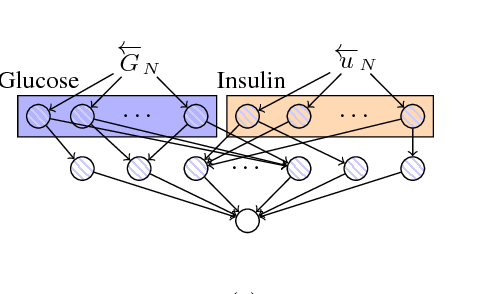
\includegraphics[width=0.7\linewidth, height=0.3\linewidth]{Images/APSDNN}
	\caption[APS DNN]{APS DNN designed by Dutta et. takes in 74 inputs of insulin and glucose. The next layers form connections between the insulin and the glucose to make predictions.[8]}
	\label{fig:apsdnn}
\end{figure}

%How is APS constructed?
The APS architecture is  the same as that discussed in Section ~\ref{apsdnn}. 
We examine the \ac{APS} controller model from Dutta et al., which has a feed-forward architecture with $2$ hidden layers and $50$ neurons each, 74 inputs and $1$ output. 
The DNN for APS takes $37$ glucose and insulin input values (for a total of 74 inputs) discretized over time and produces the next insulin values as output as shown in Figure ~\ref{fig:apsdnn}. 
 This implies that the future value is predicted based on the inputs from the previous set of values. 
The insulin and glucose values are collected from the sensors and the actuators by monitoring the patients behavior for a $30$ days. 



%Defense mechanisms
There are two distinct phases in a \ac{DNN}'s life; training and testing phase. 
During the training phase, there are three \ac{DNN}s. 
The first \ac{DNN} predicts the dose to administer. 
The other two \ac{DNN}s are defense mechanisms to prevent the patient from an insulin overdose.  
The two \ac{DNN}s are separate from the main decision making controller. 
These \ac{DNN}s are trained based on the latest 30-day patient data, which is collected by monitoring the patient to understand the standard injections for a patient over time. 

One \ac{DNN} learns a lower threshold on injection amount; the other learns an upper bound on injection amount. 
Hence, for every time of the day, based on prior patient characteristics, the minimum and the maximum values are known. 
However, the system will not detect  an adversary  who manages to always administer the maximum allowed dosage through \ac{RFDIA}. 
Hence, the attacker needs to identify inputs and  perturb them  such that the output administers the maximum allowed dosage for every injection,
  while being lower than the upper threshold to avoid detection. 
  We further elaborate this in the next section. 


\section{Attack Model}
The attacker's goal is to manipulate the sensor measurements to corrupt output without triggering alarms as shown in Figure ~\ref{fig:attackmodelphysical}. 
The attacker can use network noise or physical sensor tampering to attack the systems ~\cite{10.1145/3319535.3339815}.
 
\begin{figure}
	\centering
	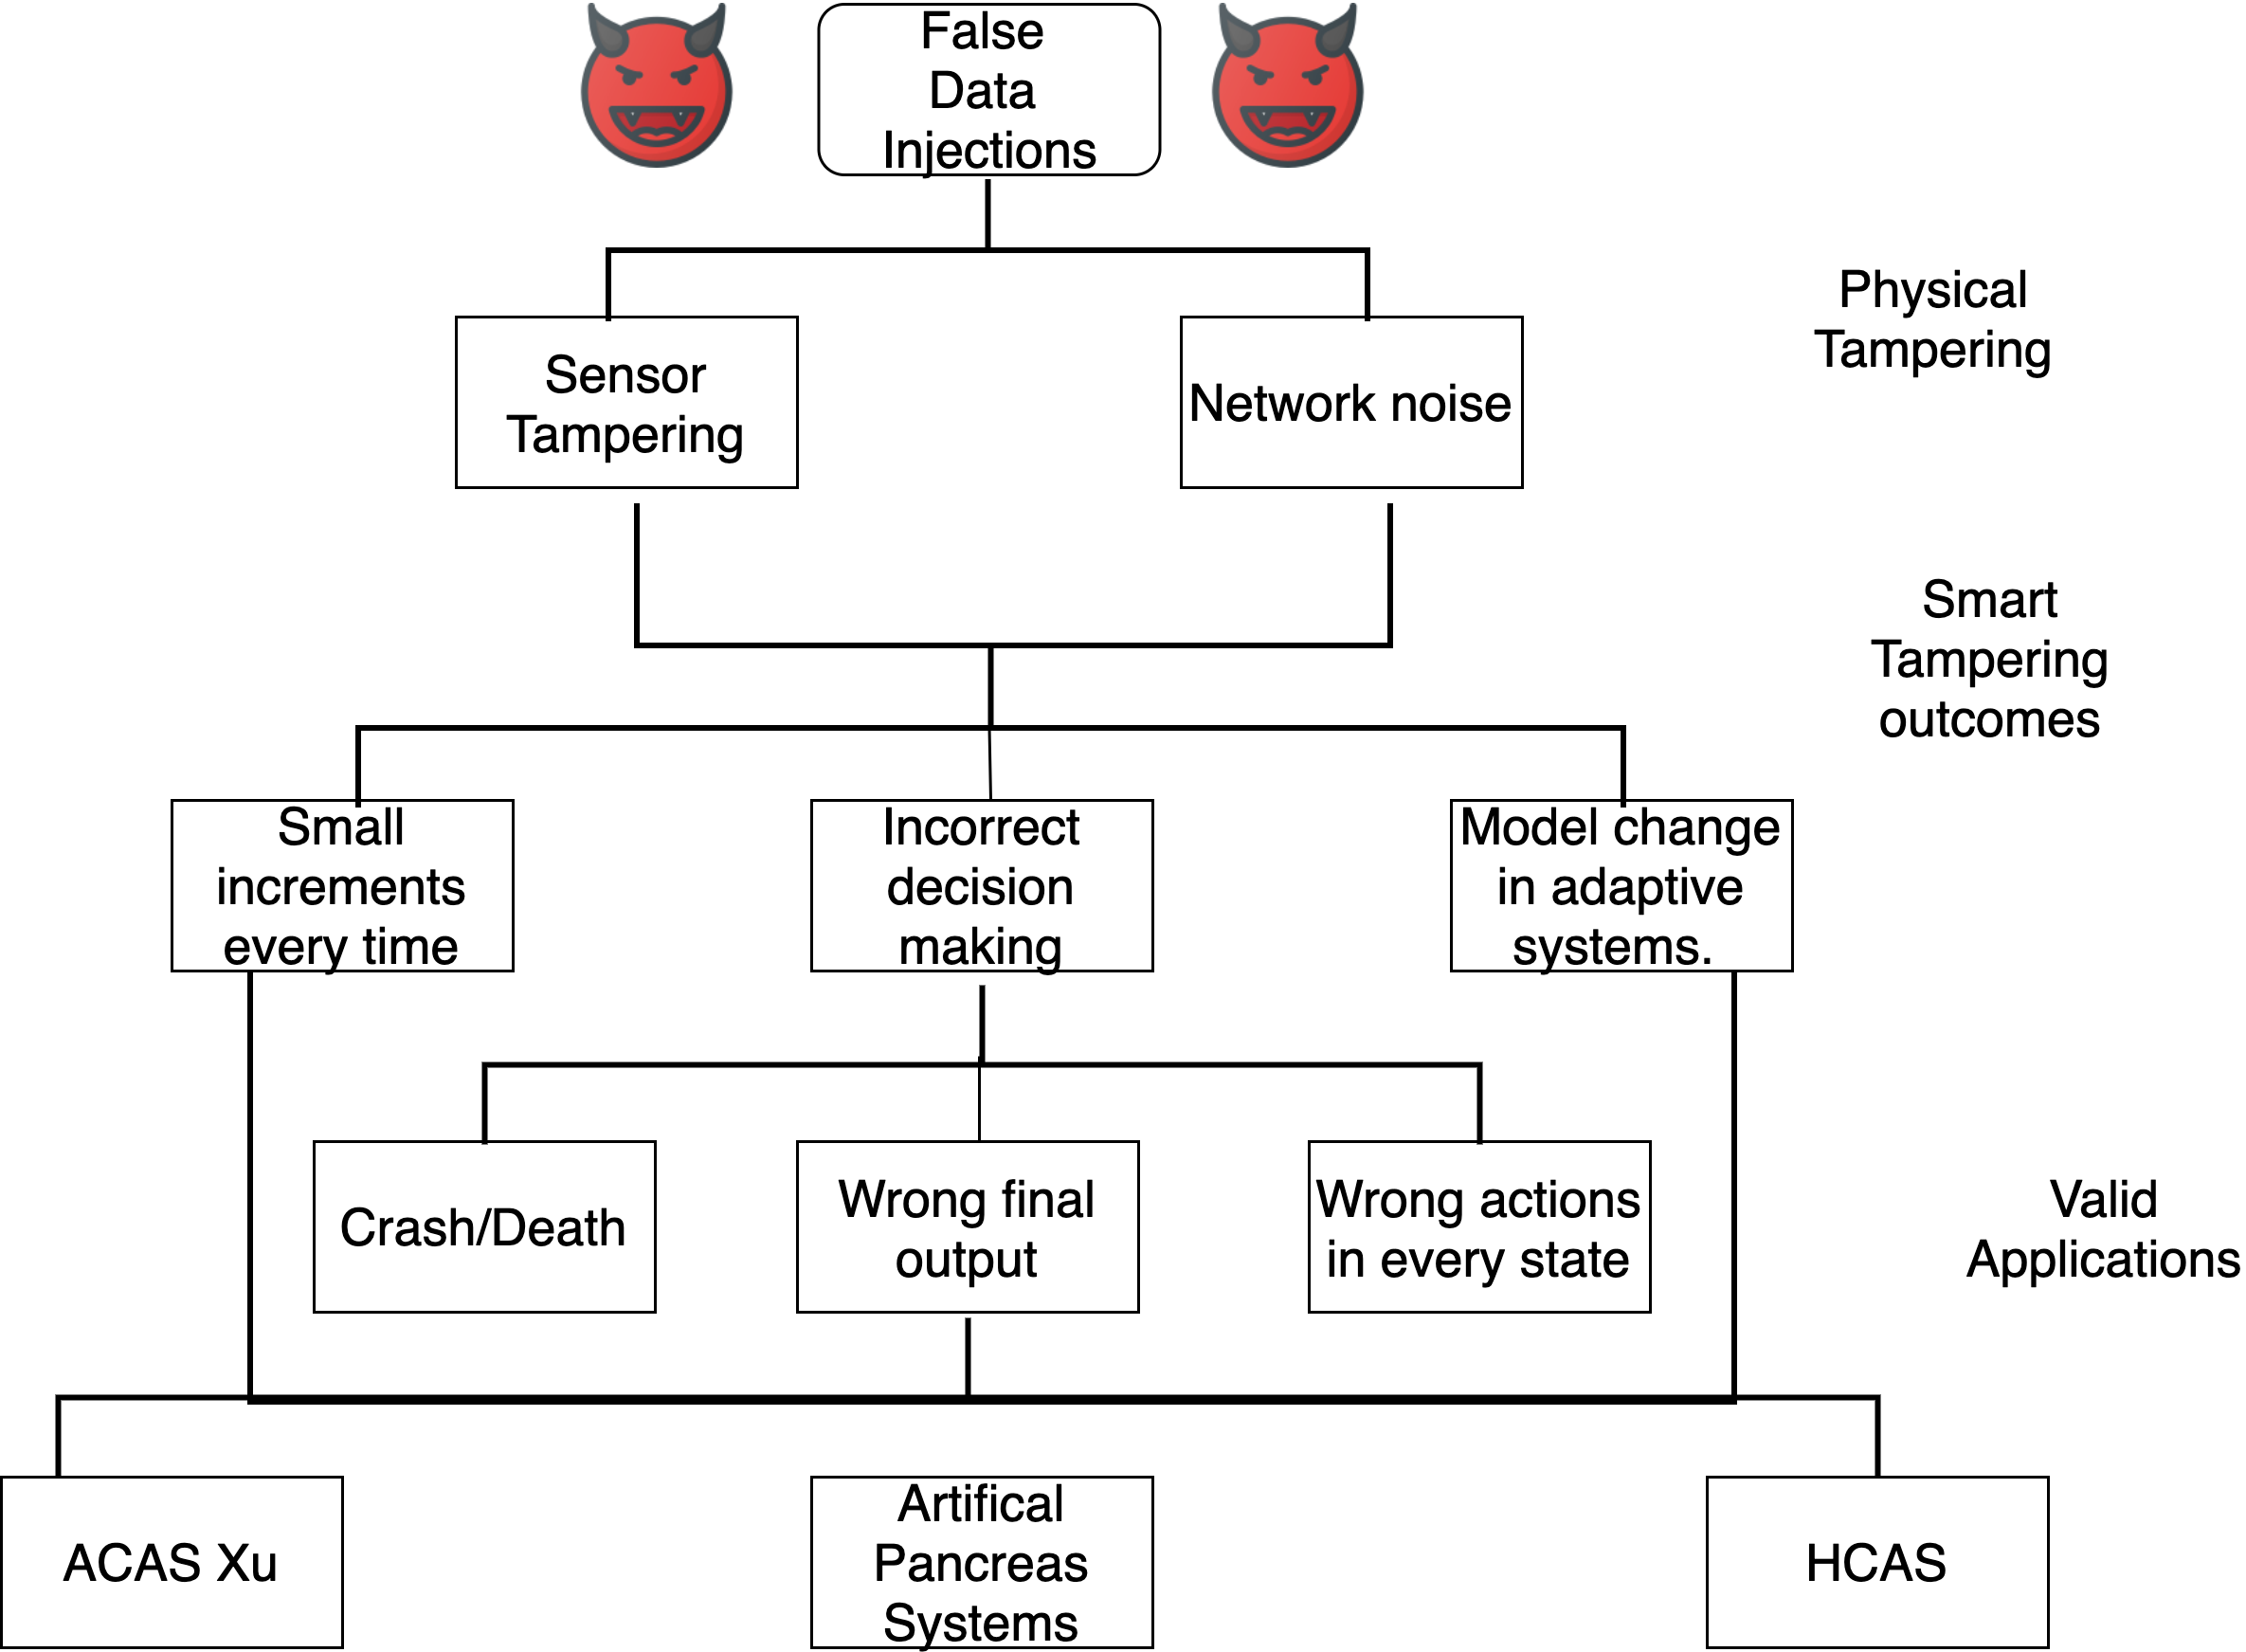
\includegraphics[width=0.7\linewidth]{Images/Attackmodelphysical}
	\caption{Attack model}
	\label{fig:attackmodelphysical}
\end{figure}

We make the following assumptions in the attack model:
\begin{enumerate}
	\item The attacker knows the precise \ac{DNN}  architecture. This information is easy to find, as the architectures are  usually specified in the  documentation. 
	\item  The weights and bias of the \ac{DNN}  are known as well through read-only access to the system.  
	\item The attacker can modify only the inputs to the model.
	\item The \ac{DNN} contains ReLU as its activation function. 
	%All three systems in this work contain ReLU.
\end{enumerate}

\subsection{Strawman attacker}
A simple way to attack the system would be to change all 74 inputs to the DNN.
 If all the inputs are changed, the final output prediction is going to be wrong. The problem in this  scenario is that 
 these inputs are collected every five minutes from the sensors attached to the patient. 
 This means that the attacker will have to conduct $74$ FDIAs every five minutes to cause a change in the output. 
 However, this is quite tedious in practice, and hence the attacker needs a better way to attack the system. 

\subsection{Sophisticated Attacker}
A more sophisticated approach to attack the system would be by perturbing a small number of inputs that cause a change in the output. 
There are two ways to proceed:

\subsubsection{Attack 1}
The attacker can randomly choose two inputs and perturb them by large amounts. 
This will indeed cause a wrong output prediction. 
However, if the input is perturbed by a large amount, the error detection mechanisms will likely recognize that there is an anomaly. 
To prevent this, the attacker can choose to perturb the two inputs by small amounts. 
However, perturbing any two random inputs by small amounts might not necessarily lead to a wrong output prediction, as shown in Chapter ~\ref{evaluation}. 

\subsubsection{Attack 2}
Adding one more layer of sophistication, the attacker can carefully chooses the inputs that can lead to wrong predictions. 
 This will be a more targeted approach for attacking the system since the input selection will not be random as before. 
However, not knowing the precise amounts by which the critical inputs should be perturbed can lead to an unsuccessful attack. 
If the perturbation is too high, it will trigger the error-detection mechanisms, 
and if it is too low, it will not affect the output as shown in Chapter ~\ref{evaluation}. 

\subsubsection{Attack 3}
The ideal attack would change a minimal number of inputs by the smallest amount possible to produce the desired change in output. 
We demonstrate that it is possible to generate this kind of attack.
 

%Our motivation for designing the technique were these different ways of attacking the system that can automatically synthesize attacks in an efficient way. 

\chapter{Challenges}
We face  the following challenges during  the design of the technique. 

\section{ Mapping DNNs to MILP}
What do I want to say ?
- DNNs when with brute force take time since we cannot keep solving every solution space. 
- Define DNN solution space mathematically
- 
DNNs are complex algorithms 
It is is difficult to use b


\section{\textbf{C1}: Finding the critical inputs}
For the sophisticated attacker to conduct \attack as described in Chapter 3, the attackers require two vital pieces. The first one is finding the critical inputs. We explain this with our motivating example of the APS system from Chapter 3. APS has 74 inputs. It is not feasible to change all inputs by False Data Injection since the attacker will have to keep changing the inputs every five minutes. Therefore, if the model architecture is known to the attacker, the goal of the attacker is to quickly locate the critical inputs. Given this is a DNN based system, it is not possible to test it for every possible input-output combination in minimal amount of time to figure out the patterns for finding the critical inputs. 

\subsubsection*{Selecting  the automated technique}
The first part is choosing a technique that allows the attacker to model a DNN and find the critical inputs through the modeling. There are multiple means of modeling the DNN, some of which are using SMT solvers, symbolic execution, MILP and many more. 
Our goal is twofold: 
\begin{enumerate}
    \item generality
    \item scalability
\end{enumerate}

APS has a  feed-forward architecture with 74 inputs whereas the other systems on which we test our technique have completely different architectures as can be observed from Table 6.1 in Chapter 6. This is due to the difference in the application domain. APS is a medical system that is much easier to reason about as compared to our other test systems that are collision avoidance systems for air traffic control management.
APS has two layers and is the smallest system that we tested our technique for but we want our technique to be valid for much bigger systems as shown in Table 1. We show that MILP fulfills these two criteria by providing us generality and scalability. 


\section*{\textbf{C2}: Finding the input perturbations}
After locating the critical inputs, the next part of the challenge is to find the correct perturbations that can lead to ripples in APS. Based on Section V formulation, if the inputs in equation (1) ($x$) are perturbed by very small amounts, the effects are not observed in the final output due to the existence of K layers in the system and the ReLU activation function as shown in (3). There is not a linear mapping between the inputs and the outputs and hence, it is a challenging problem to find just the right perturbations. We show how we tackle this in our methodology using MILP. To find the correct perturbations for \attack, we run into the following challenge. 

\subsubsection*{Designing \attack specific cost function and selecting the range intervals for inputs and outputs. }
APS DNN is an architecture where K (the number of hidden layers) is 2, and the vector input $x$ consists of 74 inputs. Our attack model is that we want to perturb the inputs by the least amounts and cause deviations in the output that are not above a certain threshold. The threshold value is determined based on the specifications of the system as described in Section III. 
 Hence, our challenge here is how we design our cost function and add a range limit to the perturbations to ensure that the perturbation does not exceed the input values above or below the bounds. 















